% ==================================================
% ChristmAIs Pipeline
% Author: Lester James V. Miranda
% ==================================================

\documentclass[preview, convert={outfile=\jobname-out.png,density=300}]{standalone}

\usepackage{tikz}
\usepackage{color}
\usepackage{subfig}
\usepackage{ifthen}
\usepackage{graphicx}
\usepackage{fontawesome}

\renewcommand\familydefault{\sfdefault}

\usetikzlibrary{
    matrix,
    shapes,
    fit,
    arrows,
    positioning,
    calc,
    backgrounds,
    shadows.blur,
    shapes.geometric,
}



\begin{document}
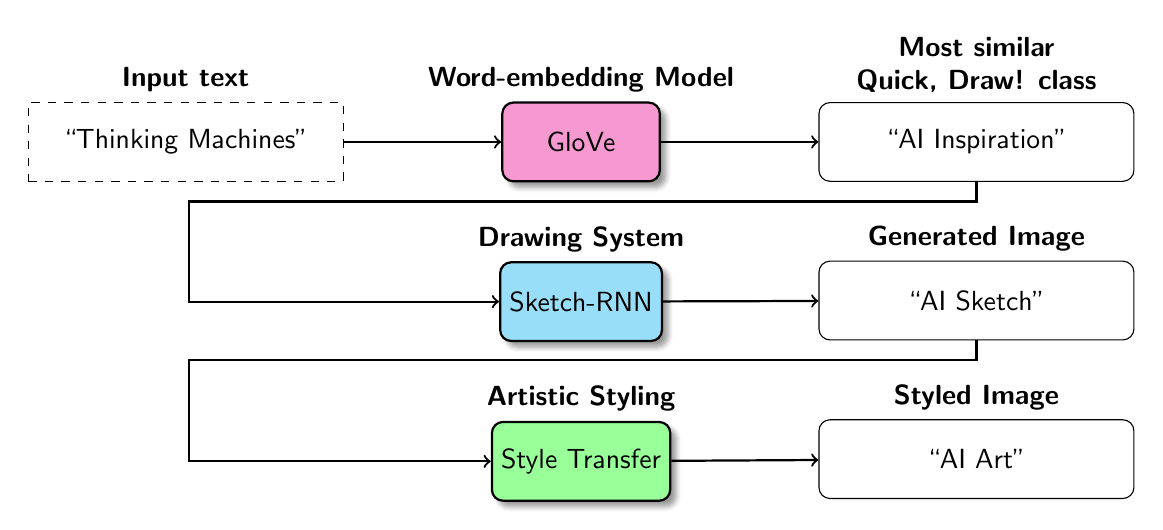
\begin{tikzpicture}[
    node distance= 1cm and 2cm,
    module/.style={draw, thick, rounded corners, text=black, align=center,
                minimum width=2cm,minimum height=1cm,fill=white, 
                blur shadow={shadow blur steps=5}},
    qd/.style={draw, rounded corners, align=center, minimum width=4cm, minimum height=1cm},
    textbox/.style={align=center, minimum width=4cm, minimum height=1cm},
]

% Input
\node[textbox,dashed,draw, label={\bfseries Input text}] at (0,0) (Input) {``Thinking Machines''};

% GloVe Embedding
\node[module,fill=magenta!40, label={\bfseries Word-embedding Model}] (WordEmbedding) [right=of Input] {GloVe};

% Quick, Draw! Class
\node[qd, label={[align=center]\bfseries Most similar\\\bfseries Quick, Draw! class}] (QDOutput) [right=of WordEmbedding] {``AI Inspiration''};

% Sketch-RNN
\node[module,fill=cyan!40, label={\bfseries Drawing System}] (DrawingSystem) [below=of WordEmbedding] {Sketch-RNN};

% Doodle
\node[qd, label={\bfseries Generated Image}] (SketchOutput) [below=of QDOutput] {``AI Sketch''};

% Style Transfer
\node[module, fill=green!40, label={\bfseries Artistic Styling}] (Styling) [below=of DrawingSystem] {Style Transfer};

% Style image
\node[qd, label={\bfseries Styled Image}] (Output) [below=of SketchOutput] {``AI Art''};


% Lines
\draw[->, thick] (Input) -- (WordEmbedding) {};
\draw[->, thick] (WordEmbedding) -- (QDOutput) {};
\draw[->, thick] (QDOutput.south) |- ++(-10cm,-0.25cm) |- (DrawingSystem.west) {};
\draw[->, thick] (DrawingSystem) -- (SketchOutput) {};
\draw[->, thick] (SketchOutput.south) |- ++(-10cm,-0.25cm) |- (Styling.west) {};
\draw[->, thick] (Styling) -- (Output) {};

\end{tikzpicture}
\end{document}

